\section{Design \& Optimization}
\label{sec:implem}

The SFA is used in the communication between an application and the underlying PaaS framework (while the SLA, on the contrary, is used for the communication between the data centre and its clients), as shown in figure 2.

\begin{figure}[h]
\label{fig:SFABlock}
\centering
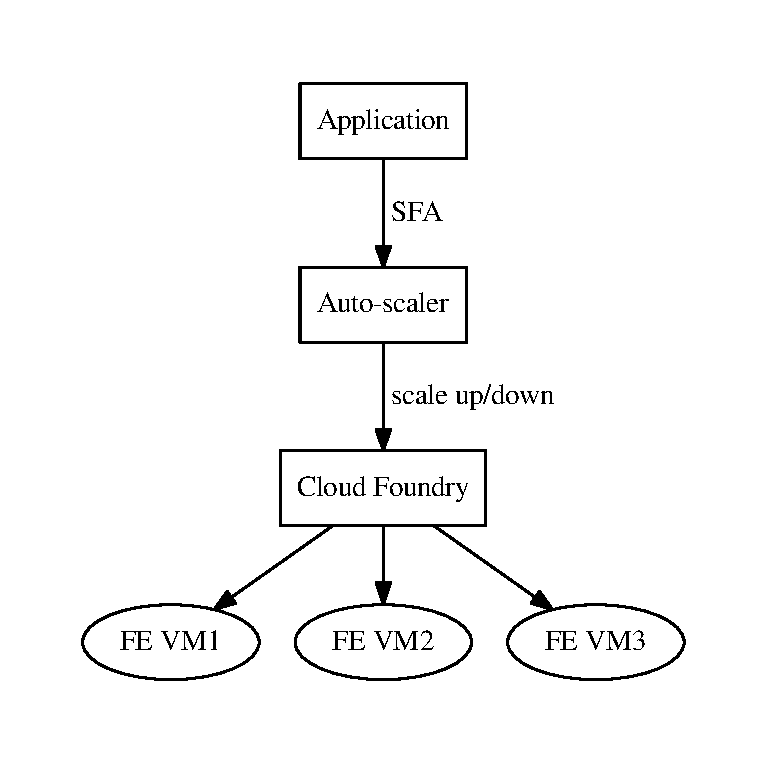
\includegraphics[width=0.6\linewidth]{generated/SFABlock.pdf}
\caption{SFA block diagram}
\end{figure}

In practice, we add a component in the Cloud Foundry stack called the "Optimizer".
This component accepts commands from the application load balancer.
Instead of just scale-up/scale-down commands as it is the case currently, we include a recommended scaling level, together with a positive deviation and a negative deviation, as described in Section~\ref{sec:sfa}.
This will let the Optimizer to optimize according to multiple criteria: 1) the energy consumption in the data centre, 2) the global happiness of the applications (the sum of all happy points granted to applications) and finally 3) the usage of renewable energies.
